\documentclass{beamer}
\usepackage{listings}
\lstset{
%language=C,
frame=single, 
breaklines=true,
columns=fullflexible
}
\usepackage{blkarray}
\usepackage{subcaption}
\usepackage{url}
\usepackage{tikz}
\usepackage{tkz-euclide} % loads  TikZ and tkz-base
%\usetkzobj{all}
\usetikzlibrary{calc,math}
\usepackage{float}
\providecommand{\brak}[1]{\ensuremath{\left(#1\right)}}
\providecommand{\pr}[1]{\ensuremath{\Pr\left(#1\right)}}
\newcommand{\myvec}[1]{\ensuremath{\begin{pmatrix}#1\end{pmatrix}}}
\newcommand\norm[1]{\left\lVert#1\right\rVert}
\renewcommand{\vec}[1]{\mathbf{#1}}
\usepackage[export]{adjustbox}
\usepackage[utf8]{inputenc}
\usepackage{amsmath}
\usepackage{tikz}
\usetikzlibrary{automata, positioning}
\usetheme{Boadilla}

\title{Ramsey 4.2 Tangent and Normal Q.16}
\author{Nelakuditi Rahul Naga - AI20BTECH11029}
\begin{document}

\begin{frame}
\titlepage
\end{frame}

\begin{frame}
\frametitle{Question}
\begin{block}{Ramsey 4.2 Tangent and Normal Q.16}
Find the equations of the circles that touch the lines:
\begin{align}
\myvec{0 & 1}\vec{x} &= 0 \label{eq:1}
\\\myvec{0 & 1}\vec{x} &= 4 \label{eq:2}
\\\myvec{2 & 1}\vec{x} &= 2 \label{eq:3}
\end{align}
\end{block}
\end{frame}

\begin{frame}
\frametitle{Solution}
\begin{block}{General Equation of a Circle}
The general equation of a circle can be expressed as:
\begin{align}
\vec{x^T}\vec{x} + 2\vec{u^T}\vec{x} + f = 0 \label{eq:4}
\end{align}
If $r$ is radius and $\vec{c}$ is the centre of the circle we have:
\begin{align}
f &=\vec{u^T}\vec{u}-r^2  \label{eq:5} \\  
\vec{c} &=-\vec{u}
\end{align}
\end{block}
\end{frame}

\begin{frame}
\frametitle{}
\begin{block}{General equation of a 2nd degree conic and point of contact of the tangent}
The general equation of a second degree can be expressed as :
\begin{align}
\vec{x^T}\vec{V}\vec{x}+2\vec{u^T}\vec{x}+f=0\label{eq:6}
\end{align}
The points of contact $\vec{q}$, of a line with a normal vector $\vec{n}$ to the conics in \eqref{eq:6} are given by:
\begin{align}
\vec{q} = \vec{V}^{-1}\brak{\kappa \vec{n}-\vec{u}} \label{eq:7} \\
\kappa = \pm \sqrt{\frac{\vec{u^T}\vec{V}^{-1}\vec{u}-f}{\vec{n^T}\vec{V}^{-1}\vec{n}}}\label{eq:8}
\end{align}
For a circle we have,
\begin{align}
\vec{V} = \vec{I}\label{eq:9} 
\end{align}
\end{block}
\end{frame}

\begin{frame}
\frametitle{}
The touch points of the circles of the form \eqref{eq:4}  with line \eqref{eq:1} are determined by:
\begin{align}
\kappa_{1} &= \pm \sqrt{\frac{\vec{u}^T\vec{u}-f}{\myvec{0 & 1 }\myvec{0 \\ 1 }}} \\
\kappa_{1} &= \pm \sqrt{\frac{r^2}{\myvec{0 & 1 }\myvec{0 \\ 1 }}} =  \pm {r}
\end{align}
Therefore we have:
\begin{align}
\vec{q_{1}} &= \pm{r}\myvec{0 \\ 1} - \vec{u}
\end{align}
Now $\vec{q_{1}}$ lies on the line \eqref{eq:1} therefore,
\begin{align}
\myvec{0 & 1}\Big(\pm{r}\myvec{0 \\ 1} - \vec{u}\Big) &= 0 \\
\implies \myvec{0 & 1}\vec{u} = \pm{r}\label{eq:10}
\end{align}
\end{frame}

\begin{frame}
\frametitle{}
The touch points of the circles of the form \eqref{eq:4}  with line \eqref{eq:2} are determined by:
\begin{align}
\kappa_{2} &= \pm \sqrt{\frac{\vec{u}^T\vec{u}-f}{\myvec{0 & 1 }\myvec{0 \\ 1 }}} \\
\kappa_{2} &= \pm \sqrt{\frac{r^2}{\myvec{0 & 1 }\myvec{0 \\ 1 }}} = \pm {r}
\end{align}
Therefore we have:
\begin{align}
\vec{q_{2}} &= \pm{r}\myvec{0 \\ 1} - \vec{u}
\end{align}
Now $\vec{q_{2}}$ lies on the line \eqref{eq:2} therefore,
\begin{align}
\myvec{0 & 1}\Big(\pm{r}\myvec{0 \\ 1} - \vec{u}\Big) &= 4 \\
\implies \myvec{0 & 1}\vec{u} = \pm{r}-4\label{eq:11}
\end{align}
\end{frame}

\begin{frame}
\frametitle{}
The touch points of the circles of the form \eqref{eq:4}  with line \eqref{eq:3} are determined by:
\begin{align}
\kappa_{3} &= \pm \sqrt{\frac{\vec{u}^T\vec{u}-f}{\myvec{2 & 1 }\myvec{2 \\ 1 }}} \\
\kappa_{3} &= \pm \sqrt{\frac{r^2}{\myvec{2 & 1 }\myvec{2 \\ 1 }}} =  \pm \dfrac{r}{\sqrt{5}}
\end{align}
Therefore we have:
\begin{align}
\vec{q_{3}} &= \pm \dfrac{r}{\sqrt{5}}\myvec{2 \\ 1} - \vec{u}
\end{align}
Now $\vec{q_{3}}$ lies on the line \eqref{eq:3} therefore,
\begin{align}
\myvec{2 & 1}\Big(\pm \dfrac{r}{\sqrt{5}}\myvec{2 \\ 1} - \vec{u}\Big) &= 2 \\
\implies \myvec{2 & 1}\vec{u} = \pm\sqrt{5}r-2\label{eq:12}
\end{align}
\end{frame}

\begin{frame}
\frametitle{}
Now we need to solve the equations \eqref{eq:10}, \eqref{eq:11} and \eqref{eq:12} written below to obtain $\vec{u}$ and $r$ :
\begin{align}
\myvec{0 & 1}\vec{u} &= \pm{r}\nonumber\\
\myvec{0 & 1}\vec{u} &= \pm{r}-4\nonumber\\
\myvec{2 & 1}\vec{u} &= \pm\sqrt{5}r-2\nonumber
\end{align}
The first two equations are consistent and give a positive solution for $r$ only when they are of the form :
\begin{align}
\myvec{0 & 1}\vec{u} &= -r\nonumber\\
\myvec{0 & 1}\vec{u} &= r-4\nonumber
\end{align}
which upon solving give :
\begin{align}
r &= 2\label{eq:13}\\
\myvec{0 & 1}\vec{u} &= -2\label{eq:14}
\end{align}
\end{frame}

\begin{frame}
\frametitle{}
Now putting $r=2$ in the third equation we have:
\begin{align}
\myvec{2 & 1}\vec{u} &= \pm2\sqrt{5}-2\label{eq:15}
\end{align}
Let us say $\vec{u} = \myvec{\alpha \\ \beta}$. Substituting $\vec{u}$ in \eqref{eq:14} we have:
\begin{align}
\myvec{0 & 1}\myvec{\alpha \\ \beta} &= -2\\
\implies \beta = -2
\end{align}
Substituting $\vec{u}$ in \eqref{eq:15} we have:
\begin{align}
\myvec{2 & 1}\myvec{\alpha \\ \beta} &= \pm2\sqrt{5} -2\\
\myvec{2 & 1}\myvec{\alpha \\ -2} &= \pm2\sqrt{5} -2\\
\implies \alpha &= \pm\sqrt{5}
\end{align}
\end{frame}

\begin{frame}
\frametitle{}
Therefore we have:
\begin{align}
\vec{u} = \myvec{\pm\sqrt{5} \\ -2}
\end{align}
Hence the value of $f$ is given by:
\begin{align}
f &=\vec{u}^T\vec{u}-r^2\\
f &= \myvec{\pm\sqrt{5} & -2}\myvec{\pm\sqrt{5} \\ -2} - 2^2\\
f &= 5
\end{align}
Hence the tangent circles are given by the equations:
\begin{align}
\vec{x^T}\vec{x} + \myvec{2\sqrt{5} & -4}\vec{x} + 5 &= 0 \\
\vec{x^T}\vec{x} + \myvec{-2\sqrt{5} & -4}\vec{x} + 5 &= 0
\end{align}
\end{frame}

\begin{frame}
\frametitle{}
The illustration of the circles and the lines is shown below :
\begin{figure}[!ht]
       \centering
    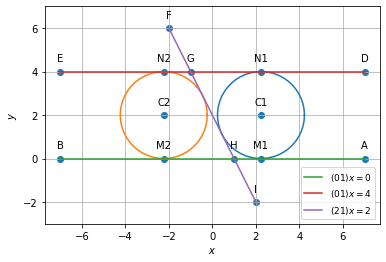
\includegraphics[width=0.8\columnwidth] {Assignment_3_Fig_1.png}
    \caption{Circles touching given lines with centres C1,C2}
    \label{Tangent circles to 3 given lines}
\end{figure}
\end{frame}

\end{document}